\documentclass[../presentation.tex]{subfiles} % Parent file
\graphicspath{{\subfix{../images/}}} % Images path

\begin{document}

\section{Datasets} % This if you want to set the gray section title

% Slide 1 ──────────────────────────────────────────────────────────────────────
\begin{frame}

	\frametitle{BraTS 2020 Dataset}
    \begin{itemize}
        \item BraTS stands for Brain Tumor Segmentation
        \item it is composed by 155 horizontal "slices" of brain MRI images for 369 patients (volumes) 
        \[155 \cdot 369 = 57195 \]
        \item we used 90\% of the dataset for training and 10\% for testing
    \end{itemize}

\end{frame}

% Slide 2 ──────────────────────────────────────────────────────────────────────
\begin{frame}
    \frametitle{BraTS 2020 Dataset}
    Images have 4 channels:
        \begin{enumerate}
            \item \textbf{T1 weighted (T1)} good for visualizing the brain but not the tumor
            \item \textbf{T1 weighted with contrast (T1c)} taken with the same tecnique as T1 but with contrast
            \item \textbf{T2 weighted (T2)} good for visualizing the edema
            \item \textbf{Fluid Attenuated Inversion Recovery (FLAIR)} improves the visualization of the edema
        \end{enumerate}
        \begin{center}
            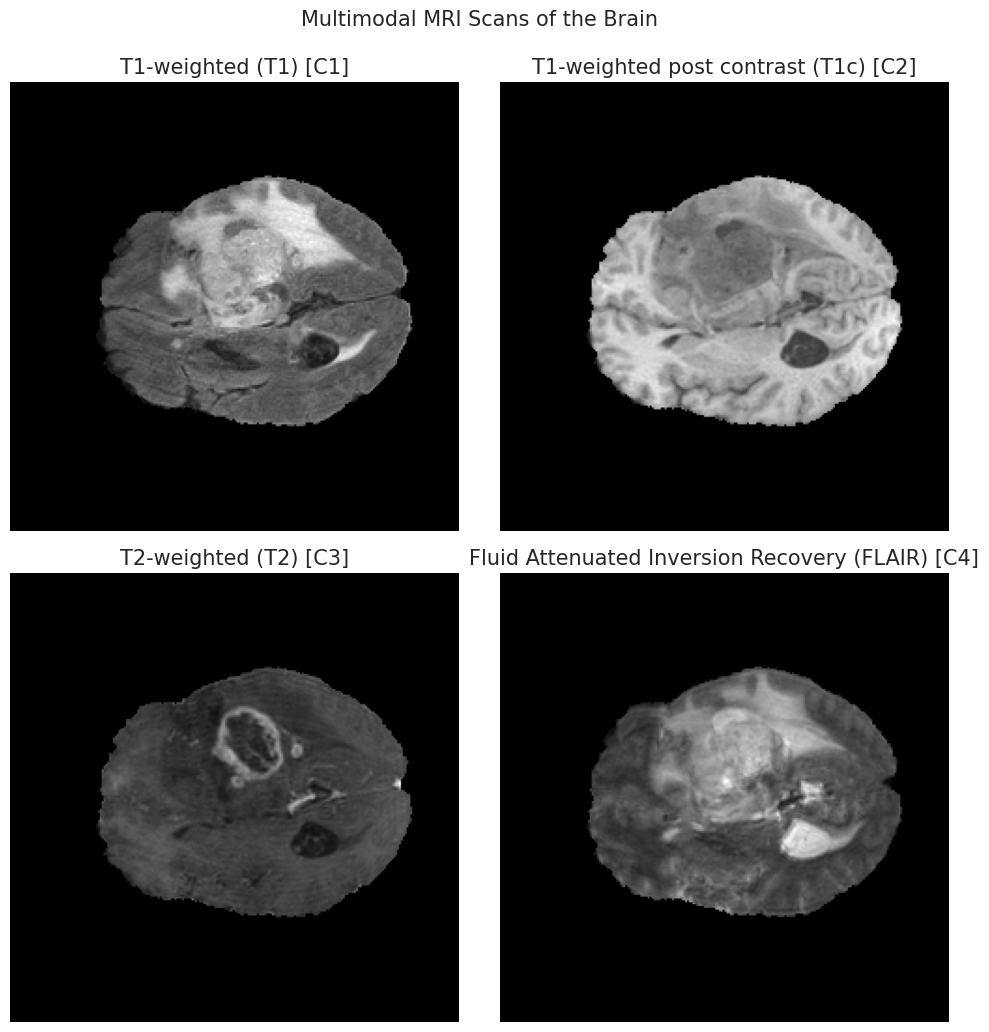
\includegraphics[width=0.4\textwidth]{segmentation_input.png}
        \end{center}
\end{frame}

% Slide 3 ──────────────────────────────────────────────────────────────────────
\begin{frame}

	\frametitle{BraTS 2020 Dataset}
    Each slice has (eventually) 3 mask labels:
    \begin{enumerate}
        \item Necrotic and Non-Enhancing Tumour Core (NCR/NET)
        \item Edema (ED)
        \item Enhancing Tumour (ET)
    \end{enumerate}
    \begin{center}
        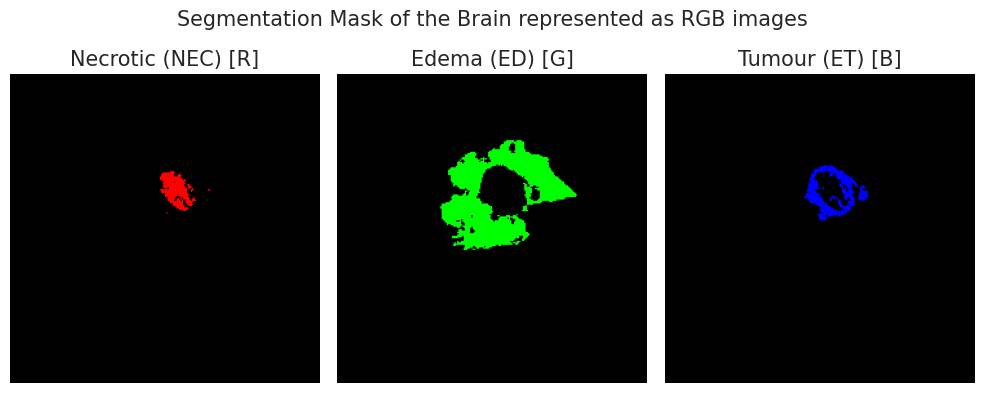
\includegraphics[width=0.65\textwidth]{segmentation_mask.png}
    \end{center}

\end{frame}

\end{document}